\section{Planning}

\begin{frame}{Discretization}{Hexagonal map}

\begin{columns}
\column{0.7\textwidth}
\begin{figure}
\centering
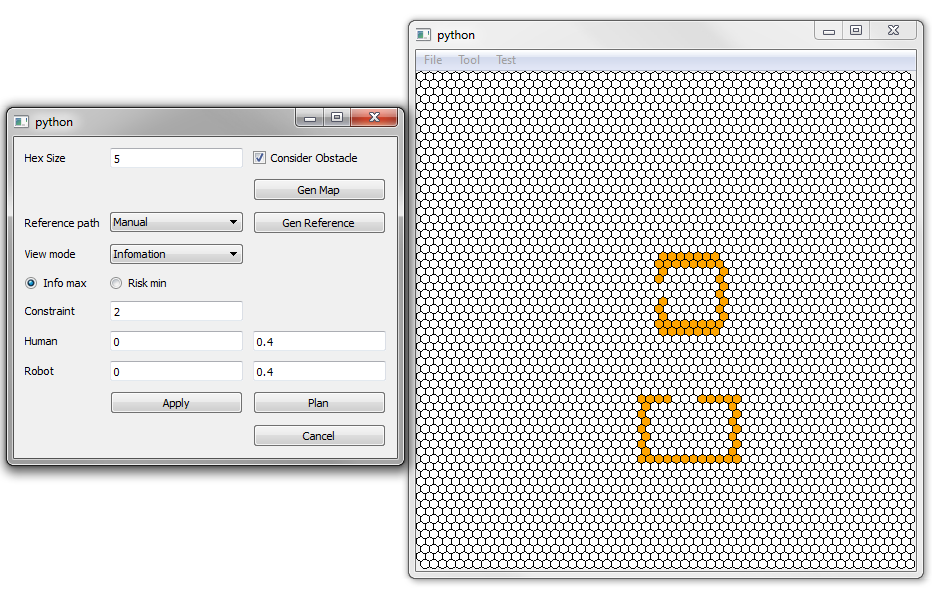
\includegraphics[width = 0.9\textwidth]{./screenshot/discretization.png}
\end{figure}

\column{0.36\textwidth}
\begin{minipage}{\textwidth}
Hexagonal discretization
\begin{figure}
\centering
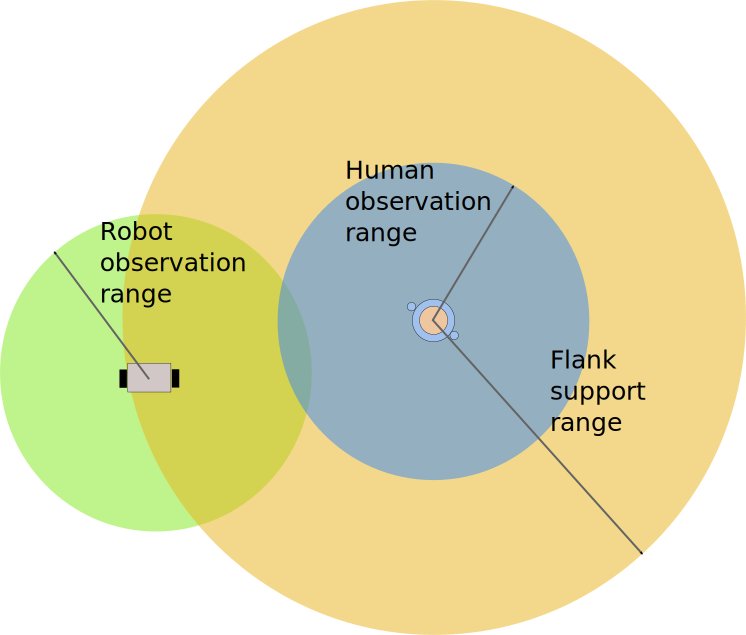
\includegraphics[width = 0.9\textwidth]{./figure/wingman}
\end{figure}
Support round observation range and motion constraint
\end{minipage}
\end{columns}

\end{frame}

\begin{frame}{View}{Information distribution}

\begin{columns}
\column{0.7\textwidth}
\begin{figure}
\centering
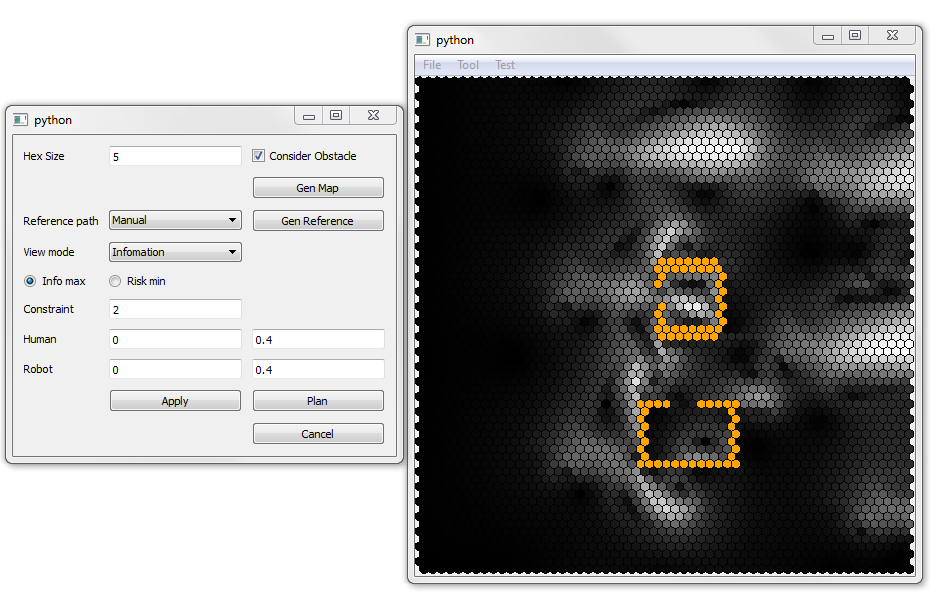
\includegraphics[width = \textwidth]{./screenshot/information_view.png}
\end{figure}

\column{0.3\textwidth}
\begin{minipage}{\textwidth}
Prior information distribution
\end{minipage}
\end{columns}

\end{frame}

\begin{frame}{View}{Enemy visibility}

\begin{columns}
\column{0.7\textwidth}
\begin{figure}
\centering
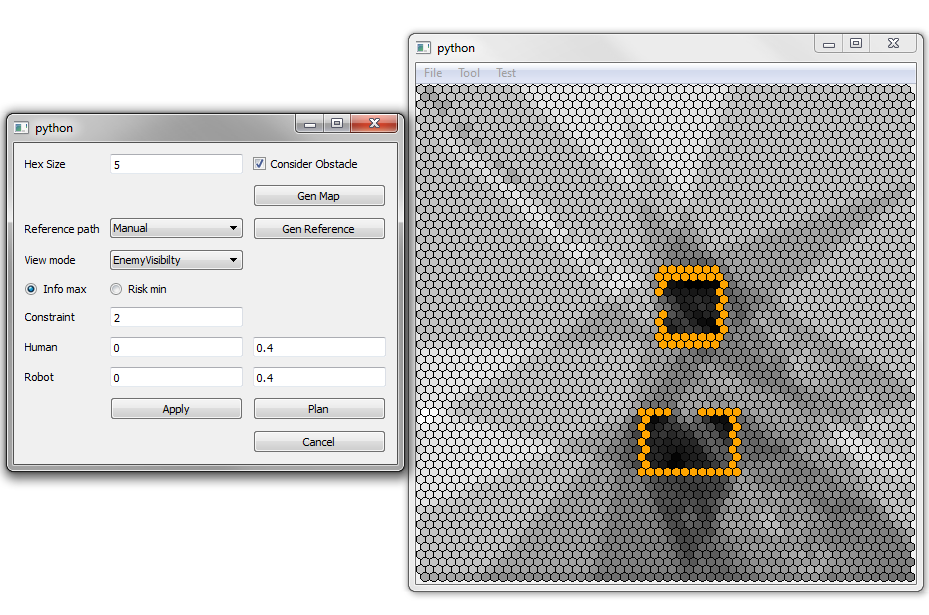
\includegraphics[width = \textwidth]{./screenshot/enemy_visibility_view.png}
\end{figure}

\column{0.3\textwidth}
\begin{minipage}{\textwidth}
The join of the visible regions of the enemies
\end{minipage}
\end{columns}

\end{frame}

\begin{frame}{View}{Position visibility}

\begin{columns}
\column{0.7\textwidth}
\begin{figure}
\centering
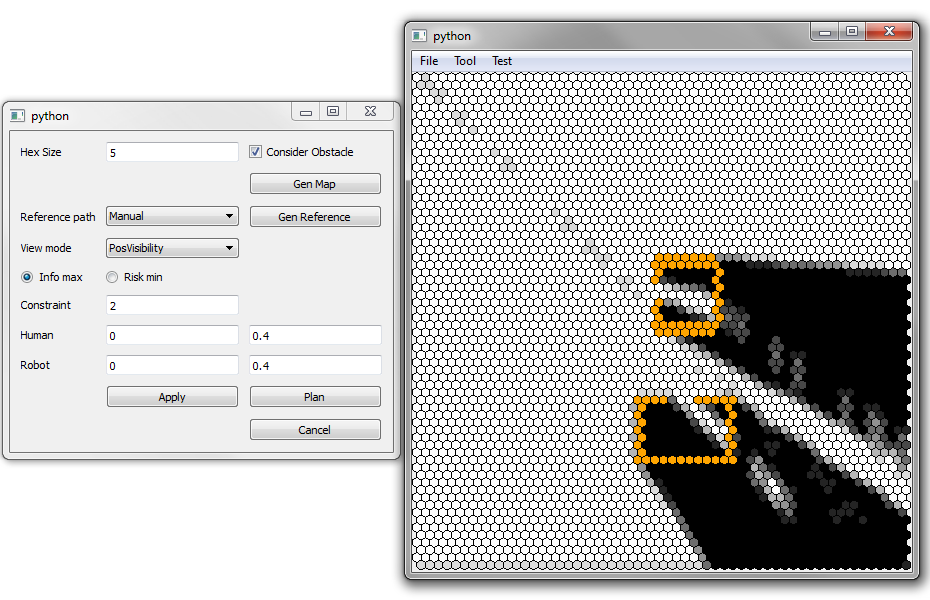
\includegraphics[width = \textwidth]{./screenshot/position_visibility_view1.png}
\end{figure}

\column{0.3\textwidth}
\begin{minipage}{\textwidth}
The visible region from standing at one position 
\end{minipage}
\end{columns}

\end{frame}

\begin{frame}{View}{Position visibility}

\begin{columns}
\column{0.7\textwidth}
\begin{figure}
\centering
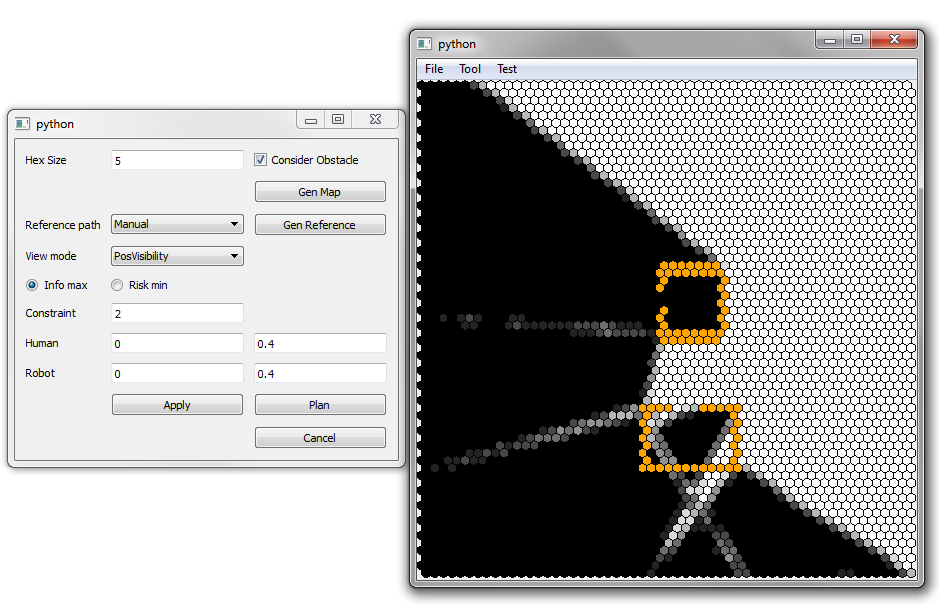
\includegraphics[width = \textwidth]{./screenshot/position_visibility_view2.png}
\end{figure}

\column{0.3\textwidth}
\begin{minipage}{\textwidth}
The visible region from standing at another position 
\end{minipage}
\end{columns}

\end{frame}

\begin{frame}{View}{Average visibility}

\begin{columns}
\column{0.7\textwidth}
\begin{figure}
\centering
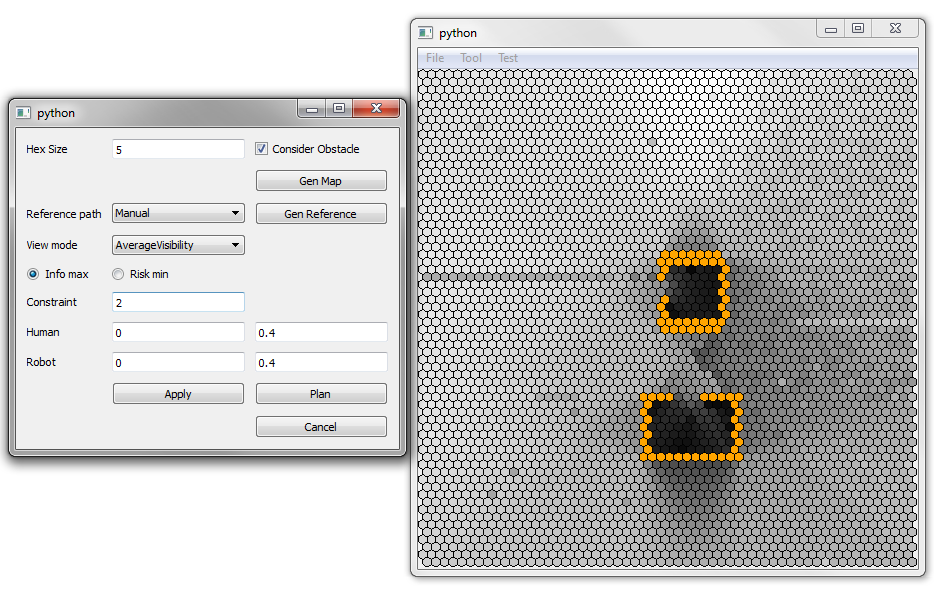
\includegraphics[width = \textwidth]{./screenshot/average_visibility_view.png}
\end{figure}

\column{0.3\textwidth}
\begin{minipage}{\textwidth}
The size of visible region from standing at each hexagon
\end{minipage}
\end{columns}

\end{frame}

\begin{frame}{Reference path}{Manual}

\begin{columns}
\column{0.65\textwidth}
\begin{figure}
\centering
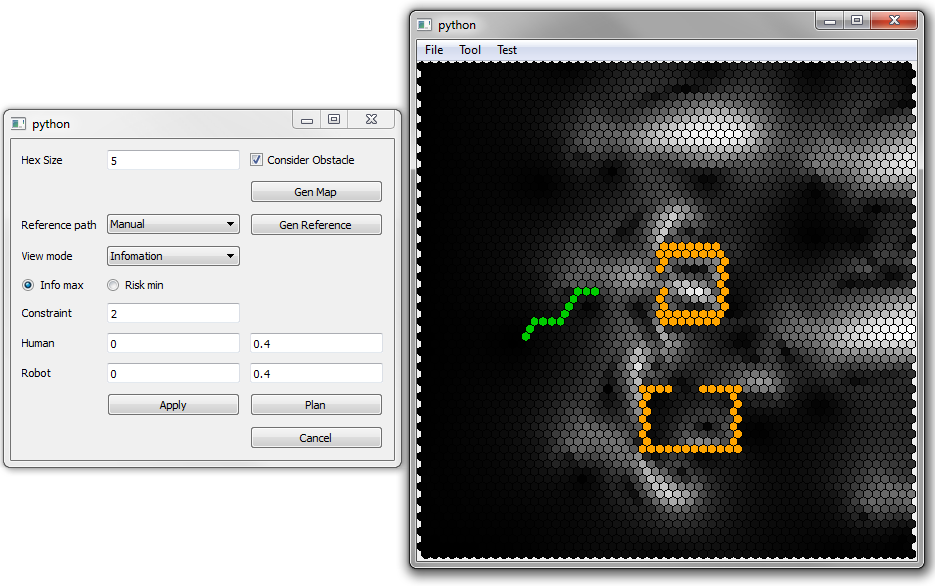
\includegraphics[width = \textwidth]{./screenshot/manual_reference_path.png}
\end{figure}

\column{0.35\textwidth}
\begin{minipage}{\textwidth}
\begin{figure}
\centering
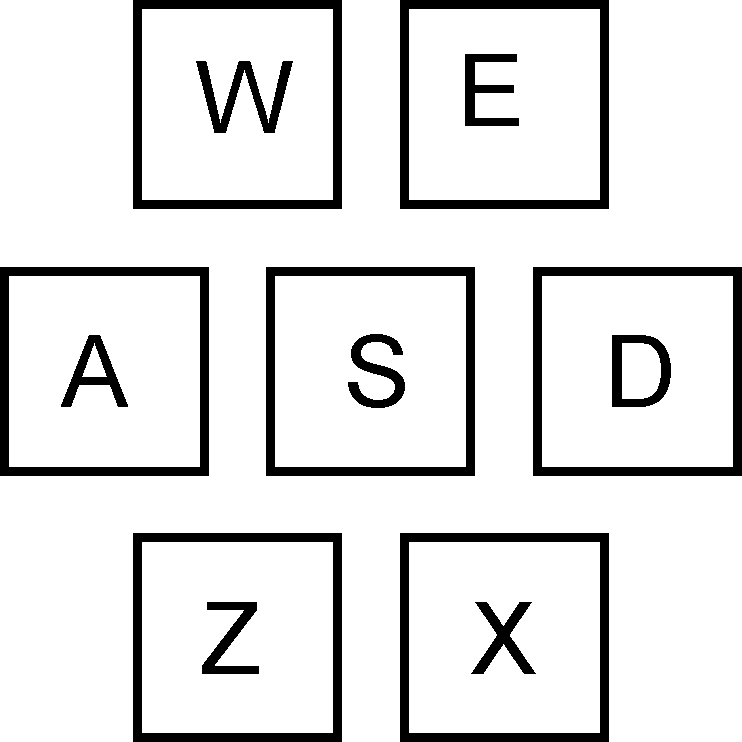
\includegraphics[width = .5\textwidth]{./figure/keyboard_op.pdf}
\end{figure}
\begin{itemize}
\item \textbf{W} - North West
\item \textbf{E} - North East
\item \textbf{A} - West 
\item \textbf{S} - Stay
\item \textbf{D} - East
\item \textbf{Z} - South West
\item \textbf{X} - South East
\end{itemize}
\end{minipage}
\end{columns}

\end{frame}

\begin{frame}{Reference path}{Quickly}

\begin{columns}
\column{0.65\textwidth}
\begin{figure}
\centering
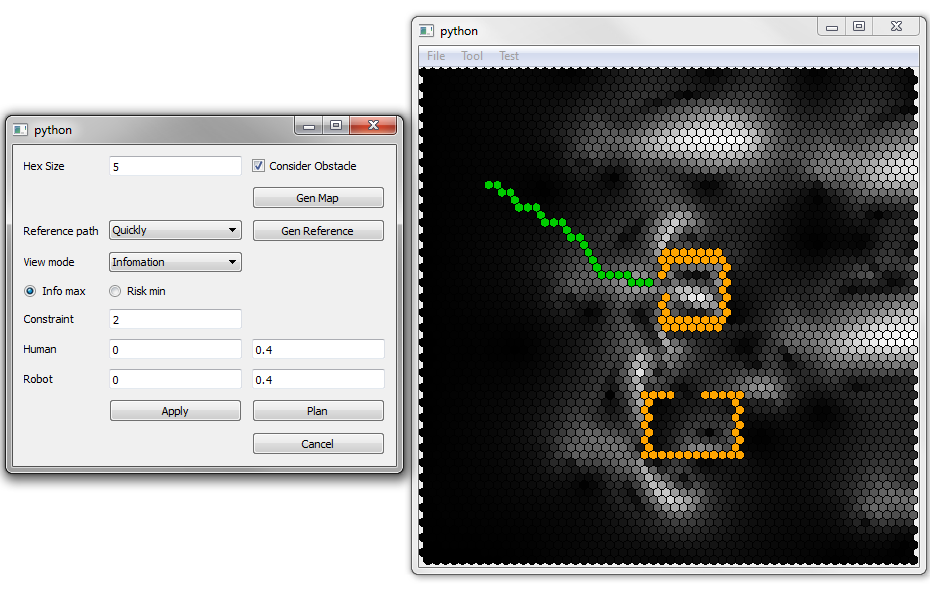
\includegraphics[width = \textwidth]{./screenshot/quickly_reference_path.png}
\end{figure}

\column{0.35\textwidth}
\begin{minipage}{\textwidth}
\emph{Metric:} maximize the information
\bigskip
Using $ A^{*} $ or visibility graph
\begin{itemize}
\item \textbf{Start point}
\item \textbf{End point}
\end{itemize}
\end{minipage}
\end{columns}

\end{frame}

\begin{frame}{Reference path}{Safely}

\begin{columns}
\column{0.65\textwidth}
\begin{figure}
\centering
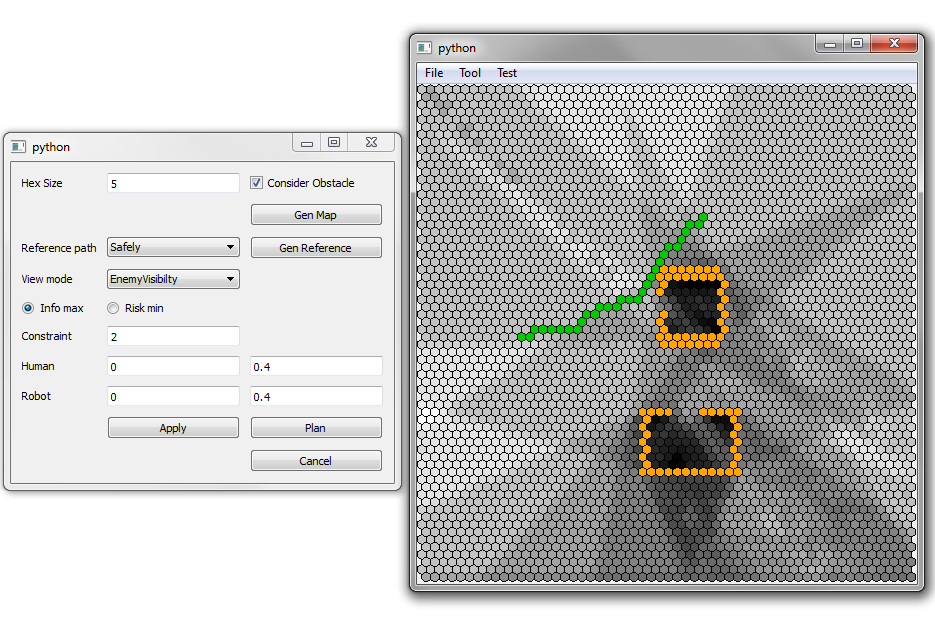
\includegraphics[width = \textwidth]{./screenshot/safely_reference_path.png}
\end{figure}

\column{0.35\textwidth}
\begin{minipage}{\textwidth}
\emph{Metric:} minimize the visibility of the enemies
\bigskip
Using $ A^{*} $
\begin{itemize}
\item \textbf{Start point}
\item \textbf{End point}
\end{itemize}
\end{minipage}
\end{columns}

\end{frame}

\begin{frame}{Path planning}{Maximize information}

\begin{columns}
\column{0.7\textwidth}
\begin{figure}
\centering
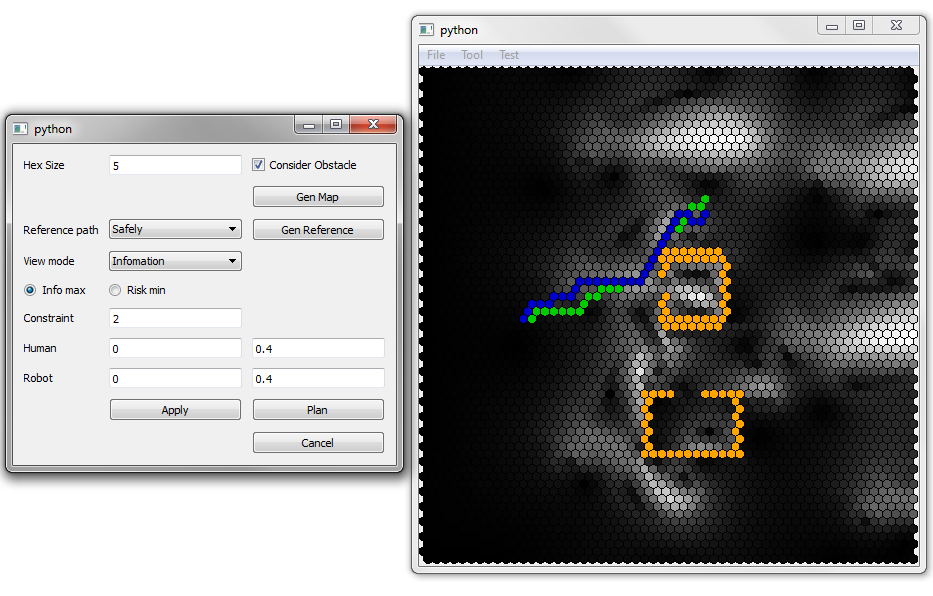
\includegraphics[width = \textwidth]{./screenshot/info_max_path.png}
\end{figure}

\column{0.3\textwidth}
\begin{minipage}{\textwidth}
\begin{itemize}
\item \emph{Informatively} (Adverb) $ \rightarrow $ maximize information
\item \emph{Motion constraint} from reference path
\end{itemize}
\end{minipage}
\end{columns}

\end{frame}

\begin{frame}{Path planning}{Minimize risk}

\begin{columns}
\column{0.7\textwidth}
\begin{figure}
\centering
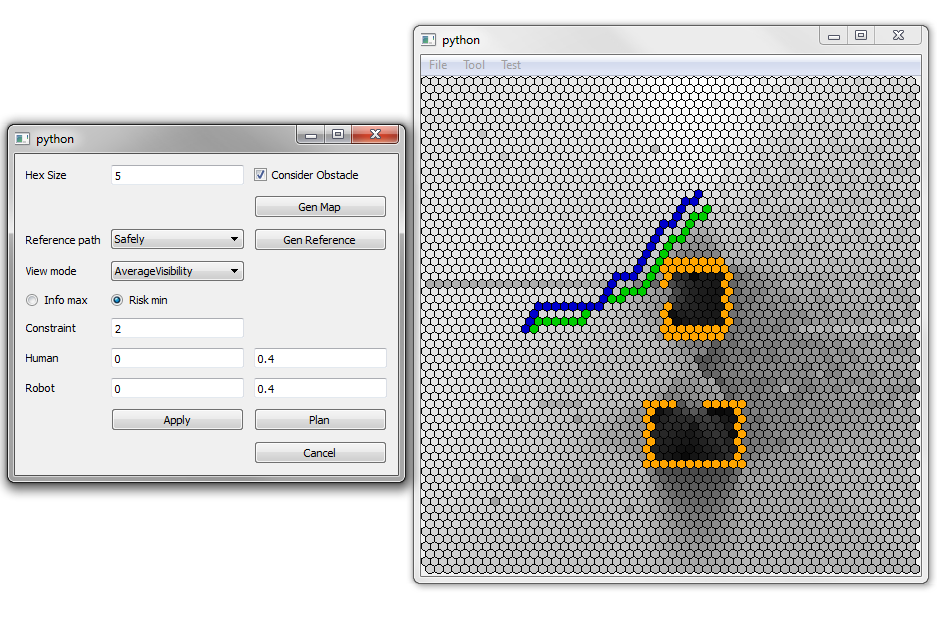
\includegraphics[width = \textwidth]{./screenshot/risk_min_path.png}
\end{figure}

\column{0.3\textwidth}
\begin{minipage}{\textwidth}
\begin{itemize}
\item \emph{Covertly} (Adverb) $ \rightarrow $ maximize visibility
\item \emph{Motion constraint} from reference path
\end{itemize}
\end{minipage}
\end{columns}

\end{frame}